%%This work may be distributed and/or modified under the conditions of the LaTeX Project Public License, either version 1.3 of this license or (at your option) any later version.
%--------------------------------------------
%%%% Copyright (C) 2021-2023 Luiz E. M. Lima (luizeduardomlima@gmail.com)
%------------------
% TEMPLATE PARA TRABALHO DE CONCLUSÃO DE CURSO
% Universidade Tecnológica Federal do Paraná - UTFPR
% Disponibilizado e adaptado pelo LAMIA - Laboratório de Aprendizado de Máquina e Images Aplicados à Indústria
% lamia-sh@utfpr.edu.br
% https://www.lamia.sh.utfpr.edu.br/ - https://github.com/lamiautfpr - https://www.instagram.com/lamiautfpr/ - 
% Campus Santa Helena
% Bacharelado em Ciência da Computação
% Projeto hospedado em: <https://github.com/lamiautfpr/TCC-Latex-COCIC-UTFPR-SH>
% Coordenador LAMIA: Thiago França Naves - naves@utfpr.edu.br
% Colaboradores: Eduardo Gasparin, João Ewerton Sousa, Paulo Vitor Souza


%% Classe de documento
\documentclass[%% Opções (^ = padrão; > = para pacotes; ¹ = somente twoside):
  a4paper,%% Tamanho de papel: a4paper, letterpaper (^), etc.
  12pt,%% Tamanho de fonte: 10pt (^), 11pt, 12pt, etc.
  oneside,%% Impressão de folhas: oneside ou twoside (^)
%   openany,%% Impressão de capítulos (¹): openany ou openright (^)
%   fleqn,%% Alinhamento de equações à esquerda (centralizado por padrão)
%   draft,%% Aparência de documento (>): draft ou final (^)
  english,%% Idioma secundário (penúltimo) (>)
  brazilian,%% Idioma primário (último) (>)
]{memoir}

%% Pacotes utilizados
\usepackage[%% Opções (^ = padrão; ¹ = somente twoside; ² = somente openany):
%   Font    = Times,%% Fonte principal: Arial (^), CM (padrão TeX) ou Times
%   Link    = TextColor,%% Cor de hyperlinks: DarkBlue (^) ou TextColor
%   Caption = Left,%% Alinhamento de legendas: Center (^) ou Left
%   Source  = Left,%% Alinhamento de fonte (referência): Center (^) ou Left
%   ABNTCit = NSB,%% Citação ABNT: AAY (NOME, ANO) (^), NRB (1) ou NSB [1]
%   BibDOI  = Icon,%% Ícone de DOI em referências: Icon ou Name (^)
%   BibURL  = Icon,%% Ícone de URL em referências: Icon ou URL (^)
%   CoverBG = On,%% Plano de fundo (capa e contracapa): On ou Off (^)
%   CoverId = All,%% Dados de identificação (capa): All ou Main (^)
%   PageNum = All,%% Numeração de páginas (partes): All, Main (^) ou None
%   TwoSide = All,%% Frente e verso (partes) (¹): All, Main (^) ou None
%   OpenPg  = Odd,%% Paginação de elementos (²): Odd ou Any (^)
%   Version = Defense,%% Versão de documento: Final (^) ou Defense
]{lamia-tcc-utfpr-sh}
\usepackage[hyperlink]{qrcode}
\usepackage{float}
\usepackage{placeins}

%% Informações do documento: descomentar para alterar
%% Importa as variáveis que contem os dados do documento (nome, autores, ano 
%% data de aprovação, banca e orientadores)
%%%% Arquivo criado por Eduardo Gasparin

%%%%%% Intruções
%%%%%% Altere apenas os campos não comentados que todos os dados de identificação do trabalho já estarão definidos

%%%% Curso(s): {Em Português}; {In English}
\Course{Ciência da Computação}{Computer Science}
%%%% Departamento(s), coordenação(ões) ou programa: {Em Português}; {In English}
\Department{Ciencia da Computação}{Computer Science}

%%%% Campus: {Cidade}
\Campus{Santa Helena}

%%%% Ano(s) (atual por padrão): [De Depósito] (opcional); {De Defesa}
\Year[2024]{2024}

%%%% Data de aprovação
%%%% Por extenso \ApprovalDate{DD de MES de ANO}{}
\ApprovalDate{XX de MesPorExtenso de 2024}{}
%%%% Abreviado \DateAbreviated{DD/MM/AAAA}{}
\DateAbreviated{21/02/2024}{}

%%%% Titulo do trabalho
\Title
{%  Em português
  Coloque aqui o titulo do trabalho em português%
}{% Em inglês
  Coloque aqui o titulo do trabalho em inglês%
}

%%%% Aluno(s) autor(es) do trabalho (de 1 a 5): {Número}; {Dados}
\Student{1}{%
  Gender   = {Male},%% Ou {Female}
  Forename = {Nome},%% Exceto último e sufixo (e.g., {José Santos da})
  Surname  = {Sobrenome},%% Último e sufixo (e.g., {Silva Júnior})
  % Email    = {seuemail@gmail.com},    %% Opcional
  % Lattes   = {0000000000010001},              %% Opcional
  % ORCID    = {0000-0000-0001-0001},           %% Opcional (CHKTEX 8)
}

%%%% Orientador(es) (de 1 a 3): {Número}; {Dados}
\Advisor{1}{%
  Gender   = {Male},%% Ou {Female}
  Title    = {\ProfCall\ \PhDCall},%% {\<T>Call}; <T>: Prof/PhD/DSc/MSc/Eng
  Fullname = {Nome do orientador},%% Conforme o Currículo Lattes
  % Email    = {advisor1@domain},%% Opcional
  % Lattes   = {0000000000020001},%% Opcional
  % ORCID    = {0000-0000-0002-0001},%% Opcional (CHKTEX 8)
}
\Advisor{2}{%
  Gender   = {Male},%% Ou {Female}
  Title    = {\ProfCall\ \PhDCall},%% {\<T>Call}; <T>: Prof/PhD/DSc/MSc/Eng
  Fullname = {Nome do coorientador},%% Conforme o Currículo Lattes
  % Email    = {advisor1@domain},%% Opcional
  % Lattes   = {0000000000020001},%% Opcional
  % ORCID    = {0000-0000-0002-0001},%% Opcional (CHKTEX 8)
}

%%%%%% Membro(s) da banca (de 3 a 6): {Número}; {Dados}
\Member{1}{%
  Gender      = {Male},%% Ou {Female}
  Title       = {Doutorado em ...},%% Por extenso ou {\<T>Call}; <T>: Prof/PhD/DSc/MSc
  Fullname    = {Nome do orientador},%% Conforme o Currículo Lattes
  Institution = {Universidade Tecnológica Federal do Paraná},%% Nome completo e por extenso
}
\Member{2}{%
  Gender      = {Male},%% Ou {Female}
  Title       = {Mestrado em ...},%% Por extenso ou {\<T>Call}; <T>: Prof/PhD/DSc/MSc
  Fullname    = {nome do membro da banca},%% Conforme o Currículo Lattes
  Institution = {Universidade Tecnológica Federal do Paraná},%% Nome completo e por extenso
}
\Member{3}{%
  Gender      = {Male},%% Ou {Female}
  Title       = {Mestrado em ...},%% Por extenso ou {\<T>Call}; <T>: Prof/PhD/DSc/MSc
  Fullname    = {nome do membro da banca},%% Conforme o Currículo Lattes
  Institution = {Universidade Tecnológica Federal do Paraná},%% Nome completo e por extenso
}
\Member{4}{%
  Gender      = {Male},%% Ou {Female}
  Title       = {Mestrado em ...},%% Por extenso ou {\<T>Call}; <T>: Prof/PhD/DSc/MSc
  Fullname    = {nome do membro da banca},%% Conforme o Currículo Lattes
  Institution = {Universidade Tecnológica Federal do Paraná},%% Nome completo e por extenso
}
% \Member{5}{%
%   Gender      = {Male},%% Ou {Female}
%   Title       = {\ProfCall\ \PhDCall},%% {\<T>Call}; <T>: Prof/PhD/DSc/MSc/Eng
%   Fullname    = {Nome Completo},%% Conforme o Currículo Lattes
%   Institution = {Instituição},%% Nome completo e por extenso
% }

%%%% Não alterar
%%%% Grau acadêmico (opção): [Número] (Obs.: (¹) automático para cada opção)
% \AcademicDegreeOption[1]%% Doutorado
% \AcademicDegreeOption[2]%% Mestrado
% \AcademicDegreeOption[3]%% Especialização
\AcademicDegreeOption[4]%% Bacharelado 
% \AcademicDegreeOption[5]%% Licenciatura
% \AcademicDegreeOption[6]%% Tecnologia
%%%%%% Grau acadêmico (¹): {Em Português}; {In English}
% \AcademicDegree{Doutorado}{Doctorate}
%%%%%% Título acadêmico (¹): {Em Português}; {In English}
% \AcademicTitle{Doutor\Gen{a}}{Doctor}
%%%%%% Tipo de documento (¹): {Em Português}; {In English}
% \DocumentType{Tese}{Thesis}
%%%% Área de concentração (Doutorado e Mestrado): {Em Português}; {In English}
% \ConcentrationArea{Térmica e Fluidos}{Thermal and Fluids}

%% Arquivo(s) de referências
\addbibresource{./Post-Textual/references.bib}

%% Processamento de entradas (itens) de listas, glossários e índices
%% Comandos \MakeAcronyms* e \MakeSymbols*: inserem as subdivisões da lista.
%%%% Lista de abreviaturas e siglas: [Arquivo de Entradas] (opcional)
\MakeAcronyms[./Pre-Textual/entries-acronyms]
%%%% Lista de símbolos: [Arquivo de Entradas] (opcional)
\MakeSymbols[./Pre-Textual/entries-symbols]
%%%% Glossário: [Arquivo de Entradas] (opcional)
\MakeGlossary[./Post-Textual/entries-glossary]
%%%% Índice remissivo
\MakeIndex%

%% Início do documento
\begin{document}%% Não comentar

%% Capa (automática)
%% Planos de fundo são inseridos na capa e numa contracapa selecionando a opção
%% CoverBG = On do pacote lamia-tcc-utfpr-sh e atribuindo argumentos válidos para grau
%% acadêmico (\AcademicDegreeOption[Número]) e campus (\Campus{Cidade}).

%% Elementos pré-textuais (frontmatter)
%% Capa, folha de rosto, errata e folha de aprovação (Não editar)
%%%% ELEMENTOS PRÉ-TEXTUAIS
%%
%% Parte que antecede o texto com informações que ajudam na identificação e na
%% utilização do trabalho.
%%
%% Observações:
%% - {Arg} argumento obrigatório de ambiente ou comando;
%% - [Arg] argumento opcional de ambiente ou comando.

%% Folha de rosto
%% Contém os elementos essenciais à identificação do trabalho, além de uma
%% licença Creative Commons (https://creativecommons.org/choose/).
%% Ambiente {TitlePage*}: aplica caixa alta no título em idioma secundário.
\begin{TitlePage}%% Argumentos (2):
[BY-NC-SA]%% Tipo de licença (BY, BY-SA, BY-ND, BY-NC, BY-NC-SA ou BY-NC-ND)
% [Texto da licença]%% Substitui o texto padrão para cada tipo de licença
%%%% Descrição do trabalho (padrão; alterar se necessário)
\DocumentTypeName\ apresentad\ifbool{Graduate}{a}{o} como requisito para obtenção do título de \StudentsTitlesList\ em \CourseName\ da \UTFPRName\ (\intl*{UTFPR}).
%%%% Ficha catalográfica (somente para Teses e Dissertações em catálogo físico)
%%%% [Arg-1]: local (pasta) do PDF (./Pre-Textual/ por padrão).
%%%% {Arg-2}: nome do PDF (em ./Pre-Textual/; modelo em ./Pre-Textual/Extras/).
% \IndexCardPDF{doc-index-card.pdf}
\end{TitlePage}

%% Errata (elemento opcional)
%% Lista dos erros ocorridos no texto, seguidos das devidas correções.
%% Ambiente {Errata*}: insere a autorreferência do documento.
% \begin{Errata}%[Título Alternativo]%% Substitui o título padrão
% %%%% Formato (com \midrule entre linhas): Página(s) & Onde se lê & Leia-se \\
% \labelcpageref{err:chpt-1,err:chpt-2,err:chpt-3,err:chpt-4,err:chpt-5,err:chpt-6} &
% capítulo{(s)}                                                                     &
% seção{(ões)} primária{(s)}                                                        \\
% \midrule%
% \pageref{err:sect}           &
% seção{(ões)}                 &
% seção{(ões)} secundária{(s)} \\
% \midrule%
% \pageref{err:ssect}         &
% subseção{(ões)}             &
% seção{(ões)} terciária{(s)} \\
% \end{Errata}

%% Folha de aprovação
%% Contém os elementos essenciais à aprovação do trabalho (sem as assinaturas).
%%%% Opção 1: gerada por meio do pacote lamia-tcc-utfpr-sh.
%%%% Ambiente {ApprovalPage*}: insere a titulação após o nome do membro.
\begin{ApprovalPage}%% Argumentos (4):
% [brazilian]%% Idioma original ou primário (brazilian ou english)
% {12 de Novembro de 2023}%% Data de aprovação (dia, mês por extenso e ano)
{\ApprovalDate}%% Data de aprovação (dia, mês por extenso e ano)
{\DateAbreviated}%% Data de aprovação (forma abreviada; mestrado e doutorado)
{\linewidth}%% Largura de linha de assinatura (graduação e especialização)
%%%%%% Descrição do trabalho (padrão; alterar se necessário)
\DocumentTypeName\ apresentad\ifbool{Graduate}{a}{o} como requisito para obtenção do título de \StudentsTitlesList\ em \CourseName\ da \UTFPRName\ (\intl*{UTFPR}).
\end{ApprovalPage}
%%%% Opção 2: gerada a partir do Sistema Acadêmico ou da secretaria.
%%%% [Arg-1]: local (pasta) do PDF (./Pre-Textual/ por padrão).
%%%% {Arg-2}: nome do PDF (em ./Pre-Textual/; modelos em ./Pre-Textual/Extras/).
% \ApprovalPagePDF{doc-approval-page.pdf}%% Não comentar (obrigatório)
%% Dedicatória
% % Dedicatória (elemento opcional)
% Texto (pessoal) em que se presta homenagem ou se dedica o trabalho.
\begin{Dedication}%% Argumentos (2):
% [Deslocamento Vertical]%% Escala de comprimento a partir da margem superior
% [Título]%% Não se aplica
%%%% Texto
Dedico este trabalho à minha família ..
\end{Dedication}%% (opcional)
%% Agradecimentos
%% Agradecimentos (elemento opcional)
%% Texto (pessoal) em que se fazem agradecimentos dirigidos àqueles que
%% contribuíram de maneira relevante à elaboração do trabalho.
\begin{Acknowledgments}%[Título Alternativo]%% Substitui o título padrão
Espaço destinado aos agradecimentos. Folha que contém manifestação de reconhecimento a pessoas e/ou instituições que realmente contribuíram com o(a) autor(a), devendo ser expressos de maneira simples.Não devem ser incluídas informações que nominem empresas ou instituições não nominadas no trabalho. Se o aluno recebeu bolsa de fomento à pesquisa, informar o nome completo da agência de fomento. Ex: Capes, CNPq, Fundação Araucária, UTFPR, etc. Incluir o número do projeto após a agência de fomento. Este item deve ser o último.

%%%% À agência de fomento (último): {Nome}; {Número/Código do Fomento}
% \FundingAgency{%
%   da \intldescr{CAPES} \textemdash\ Brasil (\intl*{CAPES})%% CAPES
% %   do \intl*{CNPq}, \intldescr{CNPq} \textemdash\ Brasil%% CNPq
% %   da Fundação Araucária \textemdash\ Brasil%% FA
% %   da \intl*{UTFPR}, \intldescr{UTFPR} \textemdash\ Brasil%% UTFPR
% }{%
%   \textemdash\ Código de Financiamento 001%% CAPES
% %   (\No\ de processo)%% CNPq
% %   (\No\ de edital, financiamento, processo ou projeto)%% FA
% %   (\No\ de edital, financiamento, processo ou projeto)%% UTFPR
% }
\end{Acknowledgments}%% (opcional)
%% Epigrafe
% %% Epígrafe (elemento opcional)
%% Texto em que se apresenta uma citação, seguida de indicação de autoria,
%% relacionada com a matéria tratada no corpo do trabalho.
%%%% Opção 1: baseada na ABNT NBR 10520 (citações diretas curtas e longas).
%%%% Ambiente {Epigraph*}: remove o formato de citação direta longa.
% \begin{Epigraph}%% Argumentos (2):
% % [Deslocamento Vertical]%% Escala de comprimento a partir da margem superior
% % [Título]%% Não se aplica
% %%%%%% Epígrafes nos idiomas primário (texto) e original (nota de rodapé)
% %%%%%% [Arg-1]: idioma (brazilian ou english).
% %%%%%% {Arg-2}: autoria.
% %%%%%% {Arg-3}: texto.
% %%%%%% [Arg-4]: nota de rodapé.
% \Citation[brazilian]{\cite[tradução]{Einstein1921}}{%
%   Até onde as leis da matemática se referem à realidade, não são certas; e até onde são certas, não se referem à realidade.
% }[%
%   \Citation[english]{\cite{Einstein1921}}{%
%     As far as the laws of mathematics refer to reality, they are not certain; and as far as they are certain, they do not refer to reality.
%   }.
% ].
% \par%
% \Citation[brazilian]{\cite[p.~37, tradução]{Asimov1950}}{%
%   Primeira Lei: um robô não pode ferir um ser humano ou, por omissão, permitir que um ser humano sofra algum mal.
%   Segunda Lei: um robô deve obedecer às ordens que lhe sejam dadas por seres humanos, exceto nos casos em que tais ordens contrariem a Primeira Lei.
%   Terceira Lei: um robô deve proteger sua própria existência desde que tal proteção não entre em conflito com a Primeira ou Segunda Leis.
% }[%
%   \Citation[english]{\cite[37]{Asimov1950}}{%
%     First Law: a robot may not injure a human being or, through inaction, allow a human being to come to harm.
%     Second Law: a robot must obey the orders given it by human beings except where such orders would conflict with the First Law.
%     Third Law: a robot must protect its own existence as long as such protection does not conflict with the First or Second Laws.
%   }.
% ].
% \end{Epigraph}
%%%% Opção 2: baseada na classe de documento memoir.
% \begin{Epigraphs}%% Argumentos (2):
% [Deslocamento Vertical]%% Escala de comprimento a partir da margem superior
% [Título]%% Não se aplica
%%%%%% Epígrafes nos idiomas primário (texto) e original (nota de rodapé)
%%%%%% [Arg-1]: idioma (brazilian ou english).
%%%%%% {Arg-2}: autoria.
%%%%%% {Arg-3}: texto.
%%%%%% [Arg-4]: nota de rodapé.
% \QItem[brazilian]{\cite[tradução]{Einstein1921}}{%
%   Até onde as leis da matemática se referem à realidade, não são certas; e até onde são certas, não se referem à realidade.
% }[%
%   \Citation[english]{\cite{Einstein1921}}{%
%     As far as the laws of mathematics refer to reality, they are not certain; and as far as they are certain, they do not refer to reality.
%   }.
% ]
% \end{Epigraphs}%% (opcional)
%% Resumo e Abstract
%% Resumo
%% Apresentação concisa dos pontos relevantes de um texto, fornecendo uma visão
%% rápida e clara do conteúdo e das conclusões do trabalho.
%% Ambiente {Abstract*}: insere a autorreferência do documento.
%%%% Estilo de fonte da chamada das palavras-chave (opcional)
% \KeywordsCallFormat{\bfseries}%% Texto normal por padrão
%%%% Palavras-chave (de 3 a 6): {Número}; {Em Português}; {In English}
\Keyword{1}{palavra-chave}{keyword}
\Keyword{2}{palavra-chave}{keyword}
\Keyword{3}{palavra-chave}{keyword}
% \Keyword{4}{palavra-chave}{keyword}

%%%% Em língua vernácula (idioma primário)
\begin{Abstract}[brazilian]%% Idioma (brazilian ou english)
O resumo deve ressaltar de forma sucinta o conteúdo do trabalho, incluindo justificativa, objetivos, metodologia, resultados e conclusão. Deve ser redigido em um único parágrafo, justificado, contendo de 150 até 500 palavras. Evitar incluir citações, fórmulas, equações e símbolos no resumo. A referência é elemento opcional em trabalhos acadêmicos, sendo que na UTFPR adotamos por não incluí-la nos resumos contidos nos próprios trabalhos. As palavras-chave e as keywords são grafadas em inicial minúscula quando não forem nome próprio ou nome científico e separados por ponto e vírgula.

\end{Abstract}

%%%% Em língua estrangeira (idioma secundário; para divulgação internacional)
\begin{Abstract}[english]%% Idioma (brazilian ou english)
Seguir o mesmo padrão do resumo, com a tradução do texto do resumo e referência, se houver, para a língua estrangeira (língua inglesa).
\end{Abstract}%% Não comentar (obrigatório)

%% Lista de algoritmos
% \PrintFloatsList{algorithm} 

%% Lista de ilustrações: figuras, fluxogramas, fotografias, gráficos e quadros
\PrintIllustrationsList{figure, flowchart, photograph, graph, tabframed}
%%%% Lista de figuras (adotar a partir de 3 itens e remover da lista geral)
% \PrintFloatsList{figure}
%%%% Lista de fluxogramas (adotar a partir de 3 itens e remover da lista geral)
% \PrintFloatsList{flowchart}
%%%% Lista de fotografias (adotar a partir de 3 itens e remover da lista geral)
% \PrintFloatsList{photograph}
%%%% Lista de gráficos (adotar a partir de 3 itens e remover da lista geral)
% \PrintFloatsList{graph}
%%%% Lista de quadros (adotar a partir de 3 itens e remover da lista geral)
% \PrintFloatsList{tabframed}

%% Lista de tabelas
\PrintFloatsList{table}

%% Lista de abreviaturas e siglas
%%%% Opção 1: makeindex; conforme o arquivo ./Pre-Textual/entries-acronyms.tex.
% \PrintAcronymsList%
%%%% Opção 2: manual; conforme o arquivo ./Pre-Textual/list-acronyms.tex.
% %%%% LISTA DE ABREVIATURAS E SIGLAS
%%
%% Elemento opcional. Consiste na relação alfabética das abreviaturas e siglas
%% utilizadas no texto, seguidas das palavras ou expressões correspondentes
%% grafadas por extenso. Recomenda-se a elaboração de lista própria para cada
%% tipo.

%% Lista de abreviaturas e siglas (inserir itens em ordem alfabética)
\begin{AcronymsList}%[Título Alternativo]%% Substitui o título padrão
\item[ABNT] Associação Brasileira de Normas Técnicas
\item[Art.] Artigo
\item[BMP] Mapa de Bits, do Inglês \ENLang*{Bitmap}
\item[Cap.] Capítulo
\item[CAPES] Coordenação de Aperfeiçoamento de Pessoal de Nível Superior
\item[CNPq] Conselho Nacional de Desenvolvimento Científico e Tecnológico
\item[CTAN] \ENLang{Comprehensive \TeX\ Archive Network}
\item[EPS] \ENLang{Encapsulated PostScript}
\item[GIF] Formato de Intercâmbio de Gráficos, do Inglês \ENLang*{Graphics Interchange Format}
\item[GIMP] Programa de Manipulação de Imagem GNU, do Inglês GNU \ENLang*{Image Manipulation Program}
\item[GNU] GNU Não é Unix, do Inglês GNU \ENLang*{is Not Unix}
\item[JPEG] \ENLang{Joint Photographic Experts Group}
\item[NBR] Norma Brasileira
\item[PDF] Formato de Documento Portátil, do Inglês \ENLang*{Portable Document Format}
\item[PNG] Gráficos Portáteis de Rede, do Inglês \ENLang*{Portable Network Graphics}
\item[PS] \ENLang{PostScript}
\item[QR] Resposta Rápida, do Inglês \ENLang*{Quick Response}
\item[Seç.] Seção
\item[TCC] Trabalho de Conclusão de Curso
\item[TUG] \ENLang{\TeX\ Users Group}
\item[UML] Linguagem de Modelagem Unificada, do Inglês \ENLang*{Unified Modeling Language}
\item[URL] Localizador Uniforme de Recursos, do Inglês \ENLang*{Uniform Resource Locator}
\item[UTFPR] Universidade Tecnológica Federal do Paraná
\end{AcronymsList}


%% Lista de símbolos
%%%% Opção 1: makeindex; conforme o arquivo ./Pre-Textual/entries-symbols.tex.
%%%% Comando \PrintSymbolsList*: insere a unidade (entre []) na margem direira.
% \PrintSymbolsList%
%%%% Opção 2: manual; conforme o arquivo ./Pre-Textual/list-symbols.tex.
% %%%% LISTA DE SÍMBOLOS
%%
%% Elemento opcional. Conjunto de sinais que substituem o nome de uma coisa ou
%% de uma ação. Elaborada conforme a ordem apresentada no texto, com o devido
%% significado.

%% Lista de símbolos (inserir itens em ordem de ocorrência)
\begin{SymbolsList}%[Título Alternativo]%% Substitui o título padrão
\item[\nu] Viscosidade cinemática, \Unit{m^2/s}
\item[\mu] Viscosidade dinâmica, \Unit{kg/{(m{}\cdot{}s)}}
\item[\rho] Massa específica, \Unit{kg/m^3}
\item[A] Área, \Unit{m^2}
\item[\pi] Constante circular (Pi), \Unit{rad}
\item[D] Diâmetro, \Unit{m}
\item[R] Raio, \Unit{m}
\item[\overline{\MrkSym}] Média temporal
\item[\langle\MrkSym\rangle] Média na seção transversal
\item[\vec{\nabla}] Operador gradiente
\item[\MrkSym^-] Passo de tempo anterior
\item[\MrkSym^+] Passo de tempo posterior
\item[\MrkSym^0] Valor inicial
\item[\MrkSym_\mathrm{G}] Fase gasosa
\item[\MrkSym_\mathrm{L}] Fase líquida
\item[\MrkSym_\mathrm{S}] Fase sólida
\item[\theta] Inclinação, \Unit{\text{\textdegree}}
\item[L] Comprimento, \Unit{m}
\item[\mathrm{Re}] Número de Reynolds
\item[V] Velocidade, \Unit{m/s}
\end{SymbolsList}


%% Sumário
%% Comando \PrintSummary*: remove o espaçamento entre partes e entre capítulos.
\PrintSummary%% Não comentar

%% Formatação de elementos textuais (mainmatter)
\Textual%% Não comentar

% Capítulo 1
\chapter{INTRODUÇÃO}\label{chp:INTRODUCAO} 
%Use referenciais sempre que necessário
Esta seção fornece uma introdução geral ao trabalho, destacando o tema e a delimitação do assunto tratado.

\section{Objetivo}\label{sec:OBJETIVOS}
%Esse texto fica como está

Expõem-se a seguir os objetivos geral e específicos que se pretende atingir com o trabalho.

\subsection{Geral}\label{sec:Geral}
%Descreva o objetivo do trabalho que é bem próximo a hipótese que você propos, veja os outros trabalhos de TCC para se inspirar

Descreve o objetivo geral do estudo, geralmente relacionado à hipótese ou propósito central do trabalho.

\subsection{Específicos}\label{sec:Especificos}
%Descreva aqui os objetivos específicos, veja os outros trabalhos de TCC para se inspirar
\begin{enumerate}
    \item Enumera objetivos específicos detalhados que serão alcançados no decorrer do trabalho;
    
    \item Objetivo especifico 2;
    
    \item Objetivo especifico 3;
    
    \item Objetivo especifico 4;
\end{enumerate}


\section{Contribuições do Trabalho}\label{sec:CONTRIBUICOES}

Descreve a principal contribuição do trabalho.

\begin{enumerate}
    \item Descreve contribuições pontuais do trabalho;
    
    \item Contribuição 2;
    
    \item Contribuição 3;
    
    \item Contribuição 4;
\end{enumerate}

\section{Justificativa}\label{sec:JUSTIFICATIVA}

Essa seção visa contextualizar a relevância do seu trabalho, mostrando por que ele é necessário e como isso pode contribuir para a resolução do problema encontrado.

\section{Delimitações do trabalho}\label{sec:DELIMITACOES}
%Você irá listar algumas delimitações utilizando uma estrutura de enumerate, veja os outros trabalhos de TCC para se inspirar
Enumera as delimitações do trabalho, indicando o que não será abordado ou comparado:

\begin{enumerate}
    \item Delimitação 1;
    \item Delimitação 2;
    \item Delimitação 3;
    \item Delimitação 4;
\end{enumerate}

% Capítulo 2
\chapter{REVISÃO DA LITERATURA}\label{chp:REVISAO}

Parte principal do trabalho, que contém a exposição ordenada e pormenorizada do assunto. É composta de revisão de literatura, dividida em seções e subseções, material e métodos e/ou metodologia e resultados, agora descritos detalhadamente. Cada seção ou subseção deverá ter um título apropriado ao conteúdo.
Deve-se utilizar sempre a terceira pessoa do singular na elaboração do texto, mantendo-se a forma impessoal

\section{Intruções para uso do documento}

De modo a facilitar a construção do texto, abaixo serão explicados os elementos necessários para a construção do texto:

\subsection{Negrito e Italico}
Colocar um texto em \textit{italico}, \textbf{negrito}.

\subsection{Listas numeradas}
Nesta lista numerada, com alguns exemplos de citação:
\begin{enumerate}
    \item Esta é uma citação ao final da linha \cite{Pressman2011},
    \item De acordo com \textcite{Pressman2011}, está é uma citação no meio da linha.
    \item Este é um exemplo de nota de rodapé do site da UTFPR\footnote{https://www.utfpr.edu.br/}
\end{enumerate}

\subsection{Listas não numeradas}
Este é um exemplo de lista não numerada:
\begin{itemize}
    \item Primeiro item da lista;
    \item Segundo item da lista;
    \item Terceiro item da lista;
\end{itemize}

\subsection{Figuras}
Na Figura \ref{fig:label-uma-figura}, temos um exemplo de figura, onde a largura dela é definida com base na largura da página (columnwidth) e com autoria própria.

\begin{figure}[htb]
	\centering
	\caption{Um exemplo de figura}
	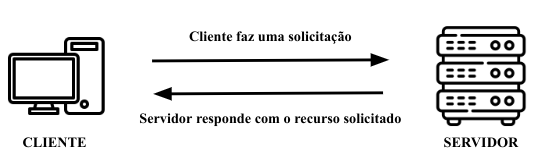
\includegraphics[width = 0.8\columnwidth]{../Images/cliente-servidor.png} 
	\newline \footnotesize \textbf{Fonte: Autoria própria (2024).}
	\label{fig:label-uma-figura}
\end{figure}

Aqui, Figura \ref{fig:outra-figura}, temos um exemplo de figura, onde a largura dela é definida com base na largura da página (columnwidth) e adaptada de uma referencia qualquer.

\begin{figure}[htb]
	\centering
	\caption{Outro exemplo de figura}
	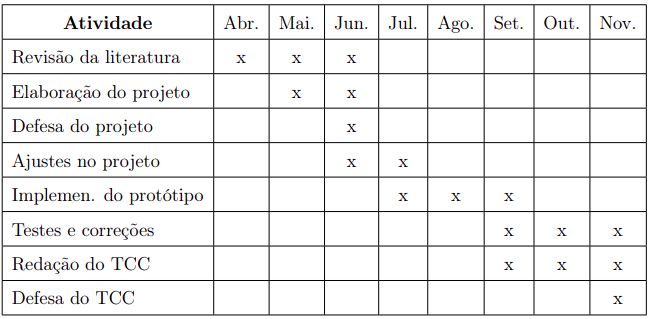
\includegraphics[width = \columnwidth]{../Images/cronograma.png} 
	\newline \footnotesize \textbf{Fonte: Adaptada de \textcite{Pressman2011, Capes2018}}
	\label{fig:outra-figura}
\end{figure}

\subsection{Tabelas}
Para elementos tabulares, deve-se usar o modelo da Tabela \ref{tab:tabela-dados}. Também é possível adicionar notas à uma tabela, para isso, use uma linha multicoluna, Tabela \ref{tab:tabela-com-nota}

\begin{table}[!htbp]
    \centering
    \caption{Tabela de dados}
    \vspace{0.1\baselineskip} 
    \label{tab:tabela-dados}
    % a primeira colula é alinhada a esquerda e as outras {2} são centralizadas
    \begin{tabularx}{\linewidth}{X *{2}{>{\centering\arraybackslash}X}}
        \hline
        \textbf{Coluna 1} & \textbf{Coluna 2} & \textbf{Coluna 3}\\ \hline
        Dados & Dados & Dados\\ 
        Dados & Dados & Dados\\
        \hline
    \end{tabularx}
    \vspace{0.1\baselineskip} 
    \newline \footnotesize \textbf{Fonte: Autoria própria (2024)}
\end{table}


\begin{table}[ht]
    \centering
    \caption{Um exemplo de tabela com nota de rodapé}
    \vspace{0.1\baselineskip} 
    \label{tab:tabela-com-nota}
    % a primeira colula é alinhada a esquerda e as outras {2} são centralizadas
    \begin{tabularx}{\linewidth}{X *{2}{>{\centering\arraybackslash}X}}
        \hline
        \textbf{Coluna 1} & \textbf{Coluna 2} & \textbf{Coluna 3}\\ \hline
        Dados & Dados & Dados\\ 
        Dados & Dados & Dados\\
        \hline
    \multicolumn{3}{l}{\textbf{Nota: Uma nota de rodapé na tabela.}}\\
    \end{tabularx}
    \vspace{0.1\baselineskip}
    \newline \footnotesize \textbf{Fonte: Autoria própria (2024)}
\end{table}

\subsection{Algoritmos e códigos}

Para inserir código, pode-se usar o \textit{lstlisting} diretamente, porem uma forma bem interessante e prática, é tratar os códigos como figuras, usando a estrutura da Figura \ref{fig:codigo-como-figura}. Neste exemplo, o código seguirá o padrão defino pela universidade, contendo a numeração de cada linha

\begin{figure}[ht]
\caption{Um json sendo representando no trabalho.}
\centering
% desse modo, tenho o codigo sendo referenciado como imagem
\begin{lstlisting}[frame=single, language=Java, breaklines=true]
{
  "Exemplo": "Um Json",
  "Objeto-1": {
    "Atributos": [
      "**"
    ],
  },
  "Objeto-2": {
    "Atributos": [
      "**"
    ],
  },
}
\end{lstlisting}
% adiciona um espaço em branco entre quadro e a legenda
\vspace{0.5\baselineskip} 
\footnotesize \textbf{Fonte: Autoria própria (2024)}.
\label{fig:codigo-como-figura}
\end{figure}
\FloatBarrier

Também disponibilizo um código em Java como exemplo na Figura \ref{fig:codigo-java}
\begin{figure}[ht]
\caption{Um código de um programa Java.}
\centering
% desse modo, tenho o codigo sendo referenciado como imagem
\begin{lstlisting}[frame=single, language=Java, breaklines=true]
// Your First Program
class HelloWorld {
    public static void main(String[] args) {
        System.out.println("Hello, World!"); 
    }
}
\end{lstlisting}
% adiciona um espaço em branco entre quadro e a legenda
\vspace{0.5\baselineskip} 
\footnotesize \textbf{Fonte: Autoria própria (2024)}.
\label{fig:codigo-java}
\end{figure}
\FloatBarrier

\subsection{Criando capitulos e seções}

Para criar diferentes níveis de seção de documento, siga o exemplo abaixo

\chapter{Cria uma seção primária}\label{chp:EXEMPLO}
% insira o texto desejado

\section{Cria uma seção secundária}
% insira o texto desejado

\subsection{Cria uma seção terciária}
% insira o texto desejado

\subsubsection{Cria uma seção quaternária}
% insira o texto desejado
% Capítulo 3
\chapter{METODOLOGIA}\label{chp:METODOLOGIA}

Deve-se colocar nessa seção, como pretende-se chegar aos objetivos definidos, como foi realizada cada etapa do trabalho. Utilize sempre que possível, figuras, tabelas e outros elementos visuais que tornem a compreensão das etapas facilitada ao leitor.
% Capítulo 4
\chapter{ANÁLISE DOS EXPERIMENTOS E RESULTADOS}\label{chp:AnaliseResultados}

%A seção foi renomeada e o texto atual não será utilizado

Nesta seção devem ser colocados os resultados obtidos, bem como as discussões acerca destes.
% Capítulo 5
\chapter{CONCLUSÃO}\label{chp:CONCLUSAO}

Faça um parágrafo resumindo o trabalho, em seguida dois outros parágrafos resumindo o sucesso da metodologia construída e dos resultados alcançados, e por fim, cite possíveis melhorias e trabalhos futuros que podem ser feitos.


%% Marcadores de PDF para capítulos subsequentes no mesmo nível de partes
% \PhantomPart%

%% Capítulo de exemplo do original
% \include{./Chapter-Example/chapter-example}

% Caso queira deixar uma pagina em branco apenas com a informação da parte e seu label:
%%\part{Nome da parte}
%%\label{part:nomelabel}

%% Formatação de elementos pós-textuais (backmatter)
%% Comando \PostTextual*: remove as seções de nível inferior às primárias do
%% sumário e dos marcadores de PDF.
\PostTextual%% Não comentar

%% Referências
\PrintReferences%% Não comentar

%% Glossário
%%%% Opção 1: makeindex; conforme o arquivo ./Post-Textual/entries-glossary.tex.
%%%% Comando \PrintGlossary*: remove o indicativo (páginas) dos itens.
% \PrintGlossary%[\bfseries]%% Estilo de fonte do termo (opcional)
%%%% Opção 2: manual; conforme o arquivo ./Post-Textual/list-glossary.tex.
% %%%% GLOSSÁRIO
%%
%% Relação de palavras ou expressões técnicas de uso restrito, ou de sentido
%% obscuro, utilizadas no texto, acompanhadas das respectivas definições.

%% Glossário (inserir itens em ordem alfabética)
\begin{Glossary}%[\bfseries]%% Estilo de fonte do termo
\item[biber] substituto do Bib\TeX\ para usuários do Bib\LaTeX.
\item[Bib\LaTeX] reimplementação completa das facilidades bibliográficas fornecidas pelo \LaTeX.
\item[Bib\LaTeX-abnt] pacote que oferece um estilo Bib\LaTeX\ que atende as regras da ABNT\@.
\item[Bib\TeX] aplicativo de gerenciamento de referências para a formatação de listas de referências no \LaTeX.
\item[componente] outro exemplo de uma entrada secundária (componente), subentrada da primária chamada pai; trata-se de uma entrada irmã de outra também secundária chamada filho.
\item[dissertação] trabalho acadêmico desenvolvido no mestrado.
\item[equilíbrio da configuração] consistência entre os componentes.
\item[filho] exemplo de uma entrada secundária (filho), subentrada da primária chamada pai.
\item[\LaTeX] conjunto de macros para o processador de textos \TeX, utilizado amplamente para a produção de textos matemáticos e científicos devido à sua alta qualidade tipográfica.
\item[memoir] classe \LaTeX\ que permite a composição de poesia, ficção, obras de não ficção e matemáticas, como livros, relatórios, artigos ou manuscritos.
\item[pai] exemplo de entrada primária (pai) que possui subentradas ou entradas secundárias (filhos).
\item[tese] trabalho acadêmico desenvolvido no doutorado.
\item[\TeX] sistema de tipografia criado por Donald E. Knuth.
\item[\lamia-tcc-utfpr-sh] modelo \LaTeX\ que permite atender os requisitos das normas definidas pela UTFPR para elaboração de trabalhos acadêmicos.
\end{Glossary}


%% Apêndices
%% Ambiente {Appendices*}: insere a folha separadora desta parte.
% \begin{Appendices}
% %%%% APÊNDICE (A)
%%
%% Texto ou documento elaborado pelo autor, de modo a complementar sua
%% argumentação, sem prejuízo da unidade nuclear do trabalho.

%% Locais (pastas) de ilustrações deste capítulo
\graphicspath{%
  {./Post-Textual/}%% Primário
%   {./Post-Textual/Illustrations/}%% Secundário (descomentar se houver)
}

\chapter{Título do Apêndice A}%
\label{chpt:apx-a}

Documentos auxiliares e/ou complementares, como legislações, estatutos, gráficos, tabelas, etc., podem ser apresentados na forma de apêndices, quando necessário.
Os apêndices, assim como os anexos, são enumerados com letras maiúsculas, por exemplo, \Cref{chpt:apx-a}.
Utilizam-se letras maiúsculas dobradas quando esgotadas as letras do alfabeto.

Apêndices complementam o texto principal do documento com informações para leitores com especial interesse no tema, devendo ser considerados leitura opcional, ou seja, o entendimento do texto principal do documento não deve exigir a leitura atenta dos apêndices.

Apêndices usualmente contemplam provas de teoremas, deduções de fórmulas matemáticas, diagramas esquemáticos, gráficos e trechos de código numérico.
Quanto a este último, um código numérico extenso não deve fazer parte do documento, mesmo como apêndice.
O ideal é disponibilizar o código numérico na Internet para os interessados em examiná-lo ou utilizá-lo, por exemplo, na plataforma \href{https://codeocean.com/}{Code Ocean\LinkIcon}, entre outras.

\section{Título de seção secundária do Apêndice A}%
\label{sect:apx-a2}

Exemplo de seção secundária de apêndice (\Cref{sect:apx-a2}).

\subsection{Título de seção terciária do Apêndice A}%
\label{ssect:apx-a3}

Exemplo de seção terciária de apêndice (\Cref{ssect:apx-a3}).

\subsubsection{Título de seção quaternária do Apêndice A}%
\label{sssect:apx-a4}

Exemplo de seção quaternária de apêndice (\Cref{sssect:apx-a4}).

\paragraph{Título de seção quinária do Apêndice A}%
\label{prgh:apx-a5}

Exemplo de seção quinária de apêndice (\Cref{prgh:apx-a5}).

\subparagraph{Título de parágrafo do \Cref{prgh:apx-a5}}%
\label{sprgh:apx-a6}

exemplo de parágrafo (divisão de seção quinária) de apêndice (\Cref{sprgh:apx-a6}).

\section{Ambientes matemáticos e atalhos úteis}%
\label{sect:math}

O \Cref{tfrm:math} apresenta os ambientes matemáticos e seus respectivos atalhos úteis em \gly*{TeX}/\gly*{LaTeX}.

\begin{tabframed}[!htbp]
\SetCaptionWidth{\textwidth}
\caption{Ambientes matemáticos e atalhos úteis}%
\label{tfrm:math}
\begin{tabularx}{\CaptionWidth}{?{}X*{3}{|>{\columncolor{shadecolor}}Y}?{}}%% CHKTEX 44
\toprule%
\multicolumn{1}{?{}Y|}{\textbf{Tipo}}                                           &
\multicolumn{1}{Y|}{\textbf{Fórmulas embutidas (no texto)}}                     &
\multicolumn{1}{Y|}{\textbf{Equações destacadas}}                               &
\multicolumn{1}{Y?{}}{\textbf{Equações destacadas e numeradas automaticamente}} \\
\midrule%
Ambiente                         &
\texttt{math}                    &
\texttt{displaymath}             &
\texttt{equation}\rlap{$^{(1)}$} \\
\midrule%
Atalho \gly*{LaTeX}                           &
\texttt{\textbackslash(\ldots\textbackslash)} &
\texttt{\textbackslash[\ldots\textbackslash]} &
{\textendash}                                 \\
\midrule%
Atalho \gly*{TeX}       &
\texttt{\$\ldots\$}     &
\texttt{\$\$\ldots\$\$} &
{\textendash}           \\
\bottomrule%
\end{tabularx}
\SourceOrNote*[]{\MathBF{^{(1)}} Versão com asterisco (\texttt{equation*}) suprime a numeração (pacote \gly*{LaTeX} \texttt{amsmath})}
\SourceOrNote{autoria própria (\YearNum)}
\end{tabframed}

% %%%% APÊNDICE (B)
%%
%% Texto ou documento elaborado pelo autor, de modo a complementar sua
%% argumentação, sem prejuízo da unidade nuclear do trabalho.

%% Locais (pastas) de ilustrações deste capítulo
\graphicspath{%
  {./Post-Textual/}%% Primário
%   {./Post-Textual/Illustrations/}%% Secundário (descomentar se houver)
}

\chapter{Cotações de Material para Montagem de um Aparato Experimental}%
\label{chpt:apx-b}

A \Cref{tab:quot} apresenta três cotações de material para montagem de um aparato experimental.

\begin{table}[!htbp]
\SetCaptionWidth{\textwidth}
\caption{Cotações de material}%
\label{tab:quot}
\begin{tabularx}{\CaptionWidth}{@{}X*{5}{,{}}@{}}
\toprule%
\multicolumn{1}{@{}c}{\textbf{Item}}        &
\multicolumn{1}{c}{\textbf{Quantidade}}     &
\multicolumn{1}{c}{\textbf{Valor 1 (R\$)}}  &
\multicolumn{1}{c}{\textbf{Valor 2 (R\$)}}  &
\multicolumn{1}{c}{\textbf{Valor 3 (R\$)}}  &
\multicolumn{1}{c@{}}{\textbf{Total (R\$)}} \\
\midrule%
Bomba centrífuga      & 1  & ^{(1)}~2500,00 & 2700,00        & 2600,00 & 2500,00 \\
Compressor rotativo   & 1  & 3000,00        & ^{(1)}~2950,00 & 3100,00 & 2950,00 \\
Manômetro diferencial & 2  & ^{(1)}~450,00  & 515,00         & 500,00  & 900,00  \\
Termopar              & 2  & 370,00         & ^{(1)}~350,00  & 400,00  & 700,00  \\
Válvula de esfera     & 2  & 43,00          & ^{(1)}~40,00   & 45,00   & 80,00   \\
Tubulação de PVC      & 5  & 10,00          & ^{(1)}~8,00    & 12,00   & 40,00   \\
Conexão de PVC        & 10 & ^{(1)}~5,00    & 6,00           & 5,00    & 50,00   \\
\midrule%
\multicolumn{5}{r}{\textbf{Total geral (R\$)}}                         & 7526,00 \\
\bottomrule%
\end{tabularx}
\SourceOrNote*[]{\MathBF{^{(1)}} Menor valor de três, empregado no total (menor valor multiplicado pela quantidade)}
\SourceOrNote{autoria própria (\YearNum)}
\end{table}

% \end{Appendices}

%% Anexos
%% Ambiente {Annexes*}: insere a folha separadora desta parte.
% \begin{Annexes}
% %%%% ANEXO (A)
%%
%% Texto ou documento não elaborado pelo autor, que serve de fundamentação,
%% comprovação e ilustração.

%% Locais (pastas) de ilustrações deste capítulo
\graphicspath{%
  {./Post-Textual/}%% Primário
  {./Post-Textual/Illustrations/}%% Secundário (descomentar se houver)
}

\chapter{Lei \No\ 9.610, de 19 de Fevereiro de 1998: Direitos Autorais / Disposições Preliminares}%
\label{chpt:anx-a}

\AddToShipoutPictureFG*{%
  \AtTextLowerLeft{%
    \setlength{\dimen1}{0pt}%
    \ifbool{@twoside}{}{\ifnumodd{\thepage}{}{\setlength{\dimen1}{\oddsidemargin-\evensidemargin}}}%
    \put(\LenToUnit{\dimen1}, 0){\includegraphics[width = \textwidth, height = \textheight, page = 1]{doc-law-n9610}}%
  }%
}\null%

\newpage%

\AddToShipoutPictureFG*{%
  \AtTextLowerLeft{%
    \setlength{\dimen1}{0pt}%
    \ifbool{@twoside}{}{\ifnumodd{\thepage}{}{\setlength{\dimen1}{\oddsidemargin-\evensidemargin}}}%
    \put(\LenToUnit{\dimen1}, 0){\includegraphics[width = \textwidth, height = \textheight, page = 2]{doc-law-n9610}}%
  }%
}\null%

\sidebar{%
  Texto completo da lei:\\[1ex]%
  \qrcode[height = 15mm]{https://www.planalto.gov.br/ccivil_03/leis/l9610.htm}%
}

% %%%% ANEXO (B)
%%
%% Texto ou documento não elaborado pelo autor, que serve de fundamentação,
%% comprovação e ilustração.

%% Locais (pastas) de ilustrações deste capítulo
\graphicspath{%
  {./Post-Textual/}%% Primário
  {./Post-Textual/Illustrations/}%% Secundário (descomentar se houver)
}

\chapter{Mapa com a Localização dos Campi da UTFPR}%
\label{chpt:anx-b}

A \Cref{fig:campi-map} apresenta um mapa com a localização dos 13 campi da \intl*{UTFPR}.

\begin{figure}[!htbp]
\SetCaptionWidth{0.7\textwidth}
\caption{Mapa com a localização dos campi da \intl*{UTFPR}}%
\label{fig:campi-map}
\savebox0{\includegraphics[width = \CaptionWidth]{fig-campi-map}}
\usebox0\llap{\raisebox{\ht0-\height}{\qrcode[height = 15mm]{https://www.utfpr.edu.br/campus}}}
\SourceOrNote{\textcite{UTFPR2017}}
\end{figure}

\section{Título de seção secundária do Anexo B}%
\label{sect:anx-b2}

Exemplo de seção secundária de anexo (\Cref{sect:anx-b2}).

\subsection{Título de seção terciária do Anexo B}%
\label{ssect:anx-b3}

Exemplo de seção terciária de anexo (\Cref{ssect:anx-b3}).

\subsubsection{Título de seção quaternária do Anexo B}%
\label{sssect:anx-b4}

Exemplo de seção quaternária de anexo (\Cref{sssect:anx-b4}).

\paragraph{Título de seção quinária do Anexo B}%
\label{prgh:anx-b5}

Exemplo de seção quinária de anexo (\Cref{prgh:anx-b5}).

\subparagraph{Título de parágrafo do \Cref{prgh:anx-b5}}%
\label{sprgh:anx-b6}

exemplo de parágrafo (divisão de seção quinária) de anexo (\Cref{sprgh:anx-b6}).

% \end{Annexes}

%% Índice remissivo
% \PrintIndex%% Não comentar

%% Fim do documento
\end{document}%% Não comentar

%% O arquivo final (PDF) pode ser convertido para PDF/A usando diversas
%% ferramentas, por exemplo:
%%   https://www.pdfforge.org/online/en/pdf-to-pdfa
